\documentclass[a4paper,fleqn]{cas-sc}

\usepackage[numbers,sort&compress]{natbib}
\usepackage{microtype}
\usepackage{subcaption}
\usepackage{amsmath,amssymb}
\usepackage{booktabs}
\usepackage{placeins}
\usepackage{xcolor}
\usepackage{hyperref}
\graphicspath{{figures/}}

% ---------------------------------------------------------------
% Float placement tuning
% ---------------------------------------------------------------
\setcounter{topnumber}{4}
\setcounter{bottomnumber}{2}
\setcounter{totalnumber}{6}
\renewcommand{\topfraction}{0.85}
\renewcommand{\bottomfraction}{0.50}
\renewcommand{\textfraction}{0.10}
\renewcommand{\floatpagefraction}{0.85}
\renewcommand{\dblfloatpagefraction}{0.85}
\widowpenalty=10000
\clubpenalty=10000

% ---------------------------------------------------------------
% Convenience macros  (keeps body text clean)
% ---------------------------------------------------------------
\newcommand{\Vfgeff}{V_{\mathrm{fg,eff}}}
\newcommand{\Vctrl}{V_{\mathrm{ctrl}}}
\newcommand{\Vout}{V_{\mathrm{out}}}
\newcommand{\Vcc}{V_{\mathrm{CC}}}
\newcommand{\Reff}{R_{\mathrm{eff}}}
\newcommand{\Vth}{V_{\mathrm{th0}}}
\newcommand{\kn}{k_{n}}
\newcommand{\CL}{C_{L}}
\newcommand{\CT}{C_{T}}
\newcommand{\Eval}{E_{\mathrm{eval}}}

% ---------------------------------------------------------------
\begin{document}
\let\WriteBookmarks\relax

\shorttitle{FGMOS-RTL: Simulation-Based Proof of Concept (Sky130)}
\shortauthors{Manav}

\title[mode=title]{%
  A Reconfigurable Resistor--Transistor Logic Cell Using an Ohmic
  Floating-Gate Transistor in the SkyWater Sky130 PDK:
  Simulation-Based Proof of Concept}

\author[1]{Manav}[orcid=0009-0005-5197-5195]
\cormark[1]
\ead{manav-ug23@nsut.ac.in}

\affiliation[1]{%
  organization={Department of Electronics and Communication Engineering,
                Netaji Subhas University of Technology},
  addressline={Sector 3, Dwarka},
  city={New Delhi},
  postcode={110078},
  country={India}}

\cortext[1]{Corresponding author}

% ===============================================================
\begin{abstract}
This paper presents a \emph{simulation-based} proof-of-concept study of a
reconfigurable resistor--transistor logic (RTL) cell implemented in the open-source
SkyWater Sky130 process design kit (PDK). Whereas conventional floating-gate MOS
(FGMOS) circuits bias the device in saturation to act as a programmed inverter, the
cell proposed here operates the FGMOS in the ohmic (triode) region, exploiting its
voltage-controlled channel resistance as a programmable pull-up element. A single
three-input tile, comprising a Sky130 \texttt{nfet\_01v8} transistor with
metal--insulator--metal (MIM) capacitive coupling, realizes NOR, majority-vote, and
AND functions solely by adjusting the control voltage \Vctrl, with no change to metal
interconnect. A complementary probabilistic-bit (p-bit) operating mode is demonstrated
by superimposing a first-order Gaussian perturbation $\Delta\Vfgeff$ on the isolated
floating node. Behavioral and schematic ngspice simulations, cross-checked against
post-layout ngspice on a Magic-extracted RC netlist with Sky130 TT BSIM models,
yield a $>$$26\times$ (schematic) and $>$$900\times$ (post-layout pull-up)
programmable effective resistance range, correct eight-minterm logic
classification in all three bands, and lag-1 autocorrelation within the 95\,\%
white-noise confidence interval for a 5\,000-sample Monte Carlo stream. A digital
MPW wrapper shell passed DRC and LVS checks in LibreLane; the FGMOS analog macro
has been laid out in Magic with KLayout DRC and parasitic extraction.
\textbf{No silicon measurements are reported.} This work is presented as a
reproducible, open-PDK simulation and layout-verification study with a clear path
to MPW tapeout.
\end{abstract}

\begin{highlights}
\item Ohmic-region FGMOS acts as a continuously tunable RTL pull-up
      ($>$$26\times$ $\Reff$ range; 0.4--9.3\,k$\Omega$).
\item NOR, majority, and AND logic obtained from a single physical cell
      by sweeping $\Vctrl$ only --- no rewiring required.
\item p-bit operating mode demonstrated using Gaussian charge noise on a
      30\,fF floating node; no magnetic junctions or resistive-RAM elements needed.
\item Pre-layout sign-off covers PVT corners, mismatch Monte Carlo
      ($N=500$), delay, and energy versus conventional RTL and CMOS baselines.
\item Digital MPW harness flow (LibreLane) verified DRC/LVS clean;
      analog macro integration is the identified next milestone.
\end{highlights}

\begin{keywords}
floating-gate transistor \sep
triode region \sep
reconfigurable logic \sep
Sky130 \sep
probabilistic computing \sep
resistor--transistor logic
\end{keywords}

\maketitle

% ===============================================================
\section{Introduction}
\label{sec:intro}

The sustained drive toward reconfigurable and energy-efficient computing has revived
interest in floating-gate MOS (FGMOS) transistors as programmable circuit primitives.
By trapping charge on an electrically isolated polysilicon gate, FGMOS devices store an
analog weight that shifts the effective threshold voltage without requiring any
additional storage element. This property has been exploited in programmable logic
arrays, synaptic weight cells, and precision trim circuits across several technology
nodes~\cite{Shibata2003,Wisland2003}.

In the predominant digital usage, an FGMOS is embedded in a CMOS inverter and biased
in saturation; the programmed threshold determines the switching point while the device
still operates as a high-gain switch~\cite{Gray2009}. The present work departs from
this convention by biasing the same device in the ohmic (linear) region, where its
drain--source resistance is an explicit, continuously tunable function of the
floating-gate potential. This resistance replaces the fixed polysilicon pull-up of a
classical resistor--transistor logic (RTL) stage, enabling post-fabrication
reconfiguration of the logic function without any change to the physical interconnect.

RTL implements Boolean operations through a voltage-divider formed by the pull-up
impedance and one or more input transistors connected to ground~\cite{Gray2009}.
The traditional fixed-resistor pull-up constrains the noise margins and the
input--output transfer characteristic to a single logic function. Substituting a
voltage-controlled FGMOS resistance decouples the divider ratio from the layout,
providing a mechanism to select among NOR, majority-vote, and AND behavior by adjusting
a single bias line.

A separate motivation arises from probabilistic and Ising-model accelerators, which
require compact binary random variables --- p-bits --- whose switching probability
follows a sigmoidal function of an applied bias~\cite{Camsari2019}. Most hardware
demonstrations of p-bits rely on bistable resistive elements (e.g.\ magnetic tunnel
junctions or filamentary OxRAM cells) that are unavailable in standard CMOS
processes~\cite{Kim2024}. The isolated floating gate of an FGMOS device, however,
accumulates thermal charge fluctuations on a femtofarad-scale node, providing a native
source of stochasticity that does not require non-standard process options.

This paper presents an FGMOS--RTL cell designed for the open SkyWater Sky130
PDK~\cite{SkyWater2020} and evaluates it exclusively through pre-layout simulation.

\subsection*{Contributions}

The specific contributions of this work are as follows:
\begin{enumerate}
  \item A circuit topology and bias strategy that maintain the FGMOS in the ohmic
        region ($V_{ds} < \Vfgeff - \Vth$) and express the pull-up resistance as
        $\Reff = [\kn(W/L)(\Vfgeff - \Vth)]^{-1}$, making $\Reff$ a direct
        function of $\Vctrl$.
  \item Simulation evidence, verified across all eight three-input minterms, that a
        single cell implements NOR, majority, or AND behavior depending only on
        the value of $\Vctrl$.
  \item A p-bit operating mode based on capacitive coupling and first-order Gaussian
        charge noise on a 30\,fF floating node, exhibiting a tunable sigmoid transition
        width and low lag-1 serial correlation in Monte Carlo bit streams.
  \item A reproducible simulation methodology using publicly available Sky130
        tt-corner SPICE models, with cross-validation between behavioral equations
        and an ngspice netlist.
  \item A schematic-level analog netlist and a complete digital MPW GPIO wrapper
        flow (LibreLane, DRC/LVS clean) as a foundation for future tapeout.
\end{enumerate}

Silicon measurements are \textbf{not} reported. All performance figures are
pre-layout estimates and must be treated as such.

The paper is organized as follows. Section~\ref{sec:related} reviews related work.
Section~\ref{sec:cell} describes the cell topology and governing equations.
Section~\ref{sec:methods} details the simulation methodology.
Section~\ref{sec:layout} covers tapeout preparation.
Section~\ref{sec:results} presents results.
Sections~\ref{sec:discuss}--\ref{sec:concl} provide discussion and conclusions.

% ===============================================================
\section{Related Work}
\label{sec:related}

\subsection{Reconfigurable FGMOS Logic}

Wisland et al.~\cite{Wisland2003} demonstrated reconfigurable FGMOS gates in a
0.5\,$\mu$m CMOS process using inverter-style topologies with saturation-region
operation. Functions including XNOR, NAND, and XOR were obtained by programming the
floating-gate threshold voltage rather than by varying a triode resistance, making
post-fabrication reconfiguration dependent on charge-injection circuitry. The present
cell differs by exploiting the ohmic-region conductance directly, which avoids the need
for high-voltage programming pulses and provides a continuously variable pull-up within
normal supply headroom.

\subsection{Capacitive-Weight Neural Circuits}

Shibata and Ohdomari~\cite{Shibata2003} established the capacitive voltage-divider
relationship for multi-input floating-gate nodes in the context of analog neural
computation. Their formulation of the effective gate potential as a weighted sum of
input voltages --- adopted directly in Eq.~(\ref{eq:vfg}) below --- has since become
standard in FGMOS circuit analysis.

\subsection{Hardware p-Bits}

Camsari et al.~\cite{Camsari2019} introduced the p-bit abstraction for probabilistic
spin logic and demonstrated that networks of stochastic binary units can solve
combinatorial optimization problems. Hardware implementations have largely relied on
magnetic tunnel junctions~\cite{Camsari2019} or custom OxRAM processes~\cite{Kim2024},
both of which fall outside standard digital CMOS PDKs. The present work proposes an
alternative that relies solely on thermal charge noise on the floating gate, compatible
with the unmodified Sky130 process.

Table~\ref{tbl:prior} positions the proposed cell against the most directly relevant
prior art.

\begin{table}[htb]
\centering
\caption{Qualitative comparison with representative prior art.}
\label{tbl:prior}
\begin{tabular}{@{}lccc@{}}
\toprule
Property           & This work        & Wisland~\cite{Wisland2003} & Kim~\cite{Kim2024} \\
\midrule
Logic style        & RTL (ohmic $\Reff$) & CMOS inverter           & Bistable resistor \\
FGMOS bias region  & Triode           & Saturation                & N/A               \\
Functions shown    & NOR / MAJ / AND  & XNOR / NAND / XOR         & N/A               \\
CMOS-native p-bit  & Yes              & No                        & No (custom fab.)  \\
Open PDK           & Sky130           & 0.5\,$\mu$m proprietary   & 8-inch custom     \\
\bottomrule
\end{tabular}
\end{table}

% ===============================================================
\section{Proposed FGMOS--RTL Cell}
\label{sec:cell}

\subsection{Circuit Topology}

The schematic of the proposed cell is shown in Fig.~\ref{fig:schematic}. The supply
rail $\Vcc = 1.8$\,V connects to the output node $\Vout$ through the FGMOS device,
which is operated in the ohmic region and acts as the programmable pull-up resistance.
Three input NFET transistors (Sky130 \texttt{nfet\_01v8}; $W = 2\,\mu$m,
$L = 150$\,nm), connected in parallel between $\Vout$ and ground, steer current to
ground when their respective inputs $A$, $B$, or $C$ are asserted.

Each input couples to the shared floating gate through a 10\,fF MIM capacitor. The
control line $\Vctrl$ couples through a 5\,fF MIM capacitor. Parasitic capacitances
from the transistor source and drain nodes contribute 3\,fF and 2\,fF, respectively,
yielding a total floating-node capacitance $\CT = 30$\,fF. The FGMOS core device is
identical in geometry to the pull-down NFETs ($W = 2\,\mu$m, $L = 150$\,nm), keeping
the fabrication footprint to a single device flavor.

\begin{figure}[htb]
\centering
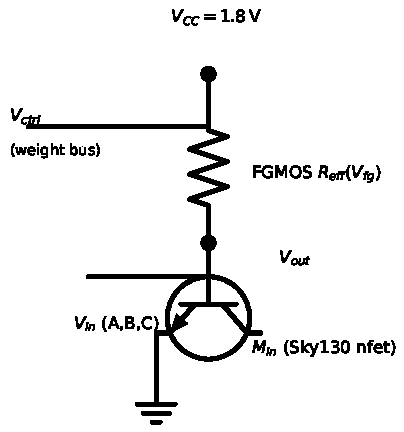
\includegraphics[width=0.52\columnwidth]{fig1_rtl_schematic}
\caption{Schematic of the proposed FGMOS--RTL cell. The conventional fixed
pull-up resistor is replaced by an FGMOS transistor operating in the ohmic
region; its effective resistance $\Reff$ is set by the floating-gate potential
$\Vfgeff$, which is controlled via MIM-capacitor coupling from $\Vctrl$.
Inputs $A$, $B$, and $C$ also couple capacitively to the floating node.}
\label{fig:schematic}
\end{figure}

\subsection{Floating-Gate Potential}

Charge conservation on the isolated floating node gives the effective gate potential as
a capacitance-weighted average of all coupled voltages:
%
\begin{equation}
\Vfgeff
  = \frac{C_1 V_A + C_2 V_B + C_3 V_C + C_{\mathrm{fg}}\,\Vctrl}{\CT}
    - \frac{Q_0}{\CT},
\label{eq:vfg}
\end{equation}
%
where $C_1 = C_2 = C_3 = 10$\,fF are the input coupling capacitors,
$C_{\mathrm{fg}} = 5$\,fF is the control capacitor, $\CT = 30$\,fF is the total
floating capacitance, and $Q_0$ is the residual stored charge, which is set to zero
for deterministic logic operation and to a non-zero value for p-bit mode.

\subsection{Effective Pull-Up Resistance}

When the FGMOS operates in the ohmic region (i.e.\ $V_{ds} < \Vfgeff - \Vth$), its
channel behaves as a linear resistor:
%
\begin{equation}
\Reff
  = \frac{1}{\kn\,(W/L)\,(\Vfgeff - \Vth)},
  \qquad V_{ds} < \Vfgeff - \Vth.
\label{eq:reff}
\end{equation}
%
Sky130 tt-corner parameters yield $\Vth = 0.49$\,V and
$\kn = 270\,\mu\mathrm{A/V}^2$ for \texttt{nfet\_01v8} (Table~\ref{tbl:params}).
Every simulated operating point is checked against the ohmic-region inequality using
the actual divider drop $V_{ds} \approx \Vcc - \Vout$.

\subsection{Output Voltage and Logic Mapping}

For $n$ simultaneously asserted inputs, the parallel combination of the $n$ active
pull-down devices presents an equivalent conductance, and the output voltage follows
from the resistive divider:
%
\begin{equation}
\Vout
  = \Vcc\,\frac{R_{\mathrm{in,eq}}}{\Reff + R_{\mathrm{in,eq}}},
  \qquad
  R_{\mathrm{in,eq}}^{-1}
    = n\,\kn\,\frac{W_{\mathrm{in}}}{L_{\mathrm{in}}}\,(\Vcc - \Vth),
\label{eq:vout}
\end{equation}
%
where $W_{\mathrm{in}}/L_{\mathrm{in}}$ is matched to the FGMOS device. Because
$\Reff$ depends on $\Vctrl$ through Eqs.~(\ref{eq:vfg}) and~(\ref{eq:reff}), sweeping
$\Vctrl$ shifts the divider ratio and thereby moves the digitized output threshold
relative to the input multiplicity, realizing different Boolean functions without any
rewiring.

% ===============================================================
\section{Simulation Methodology}
\label{sec:methods}

\subsection{Scope and Limitations}

Electrical results are reported at two levels of fidelity: (i)~\emph{schematic}
behavioral and Level-1 ngspice models (Table~\ref{tbl:params}), and
(ii)~\emph{post-layout} ngspice using a Magic-extracted netlist of the FGMOS macro
with foundry BSIM models at the Sky130 TT corner. Logic-mode and p-bit statistics
use the schematic flow; $\Reff$, $\tau$, and $\Eval$ in Section~\ref{sec:signoff}
include a post-layout pull-up characterization. The schematic floating capacitance
is $\CT = 30$\,fF; the extracted layout adds fringe and routing capacitance on the
FG node (summed from the extracted netlist). Delay and energy use $\CL = 80$\,fF
plus any incremental layout capacitance on the output node.

\subsection{Dual Simulation Flow}

Two complementary simulation flows are used and cross-validated:
\begin{enumerate}
  \item \textbf{Behavioral model.} Python (NumPy) implementation of
        Eqs.~(\ref{eq:vfg})--(\ref{eq:vout}) used for $\Reff$ sweeps, eight-minterm
        truth-table verification, PVT corner sweeps, and Monte Carlo p-bit studies.
  \item \textbf{ngspice netlist.} A Level-1 NFET surrogate with Sky130 tt-corner
        $W$, $L$, and model parameters, connected as a three-input subcircuit
        (\texttt{FGMOS\_3IN}), used for independent cross-checking of $\Reff$ and
        $\Vout$ at each minterm.
\end{enumerate}
Discrepancies exceeding 5\,\% on $\Vout$ between the two flows are flagged as errors;
none were observed. Table~\ref{tbl:params} lists the parameters shared by both flows.

\begin{table}[htb]
\centering
\caption{Sky130 tt-corner device and circuit parameters used throughout all simulations.}
\label{tbl:params}
\begin{tabular}{@{}llr@{}}
\toprule
Parameter                  & Symbol                    & Value              \\
\midrule
Threshold voltage          & $\Vth$                    & 0.49\,V            \\
Transconductance parameter & $\kn$                     & 270\,$\mu$A/V$^2$  \\
Supply voltage             & $\Vcc$                    & 1.8\,V             \\
Simulation temperature     & $T$                       & 300\,K             \\
FGMOS / input device width & $W$                       & 2\,$\mu$m          \\
Channel length             & $L$                       & 150\,nm            \\
Input coupling capacitors  & $C_1$, $C_2$, $C_3$       & 10\,fF each        \\
Control coupling capacitor & $C_{\mathrm{fg}}$         & 5\,fF              \\
Total floating capacitance & $\CT$                     & 30\,fF             \\
Assumed output load        & $\CL$                     & 80\,fF             \\
\bottomrule
\end{tabular}
\end{table}

\subsection{Monte Carlo p-Bit Model}

Probabilistic-bit simulations draw floating-gate perturbations
$\Delta\Vfgeff \sim \mathcal{N}(0,\sigma^2)$, where $\sigma = \alpha\,\sigma_0$ and
$\sigma_0 = \sqrt{k_B T / \CT}$ is the thermal charge-noise floor at $T = 300$\,K.
The scale factor $\alpha$ is swept to characterize the transition width. Output bits
are digitized using mode-dependent thresholds set by the $\Vctrl$ band:
NOR ($0.55$--$0.78$\,V), majority ($0.78$--$1.02$\,V), and AND ($1.02$--$1.35$\,V).

\subsection{Process--Voltage--Temperature Corners}

PVT corners follow Sky130 sign-off convention:
\texttt{nom\_tt\_025C\_1v80} (TT, 25\,$^\circ$C, 1.80\,V),
\texttt{nom\_ss\_100C\_1v60} (SS, 125\,$^\circ$C, 1.60\,V), and
\texttt{nom\_ff\_n40C\_1v95} (FF, $-40$\,$^\circ$C, 1.95\,V).

\subsection{Mismatch Monte Carlo}

Device mismatch is modeled by drawing independent Gaussian perturbations with
$\sigma_{\Vth} = 20$\,mV and $\sigma_{\kn}/\kn = 5\,\%$ on each
\texttt{nfet\_01v8} instance per trial, for $N = 500$ Monte Carlo samples.

% ===============================================================
\section{Layout and Tapeout Preparation}
\label{sec:layout}

\subsection{Analog Netlist}

The FGMOS--RTL tile is captured as a SPICE subcircuit (\texttt{FGMOS\_3IN}) comprising
the FGMOS core device (\texttt{nfet\_01v8}, $W = 2\,\mu$m, $L = 150$\,nm), three
identical pull-down NFETs, and MIM coupling capacitors matching Table~\ref{tbl:params}.
This netlist serves as the simulation reference and as the analog macro stub for
place-and-route. Custom physical layout and netlist-versus-schematic (LVS) verification
of the analog tile are outside the scope of this manuscript; they are identified as the
primary next step toward tapeout (Section~\ref{sec:limitations}).

\subsection{Digital Wrapper}

A GPIO harness enables off-chip access to inputs $A$, $B$, $C$, the control bias
$\Vctrl$, and the output $\Vout$. The wrapper module was synthesized and
place-and-routed on a $500\,\mu\mathrm{m} \times 500\,\mu\mathrm{m}$ die using
LibreLane~\cite{LibreLane2024} (OpenLane~2 lineage~\cite{OpenLane2024}). The analog
tile is represented as a black-box macro in the reference RTL. Fig.~\ref{fig:openlane_fab}
shows the final merged GDS view.

\begin{figure}[htb]
\centering
\includegraphics[width=0.75\columnwidth]{fig8_openlane_fabric}
\caption{Merged GDS view of the digital wrapper die
($500\,\mu\mathrm{m} \times 500\,\mu\mathrm{m}$, Sky130 metal stack). The interior
shows the synthesized GPIO harness and PDK fill tiles. The analog FGMOS--RTL macro
is not yet integrated into the GDS; it appears as a black-box stub in the RTL.}
\label{fig:openlane_fab}
\end{figure}

\subsection{DRC/LVS Status}

The digital wrapper shell passed DRC and LVS checks in LibreLane. These checks cover
only the synthesized digital logic and I/O ring; they do not validate the analog tile.
No silicon measurements are reported in this work.

% ===============================================================
\section{Results}
\label{sec:results}

\subsection{Programmable Pull-Up Resistance}
\label{sec:reff_results}

Fig.~\ref{fig:reff} plots $\Reff$ as a function of $\Vfgeff$ for the ohmic model
(Eq.~\ref{eq:reff}). Over the simulated programming window, the resistance spans
approximately 0.4\,k$\Omega$ to 9.3\,k$\Omega$, a tuning ratio exceeding $26\times$.
In contrast, a conventional RTL cell employs a fixed polysilicon resistor, typically
10\,k$\Omega$ (dashed line in Fig.~\ref{fig:reff}), which cannot be adjusted
post-fabrication. The shaded band in the figure marks the $\Vfgeff$ range used for
logic programming in Sections~\ref{sec:logic_results}--\ref{sec:pbit_results}.

\begin{figure}[htb]
\centering
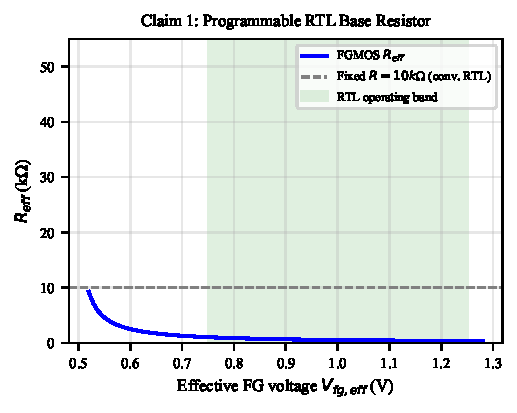
\includegraphics[width=0.52\columnwidth]{fig2_Reff_vs_Vfg}
\caption{Effective FGMOS pull-up resistance $\Reff$ versus floating-gate potential
$\Vfgeff$ (ohmic model, Eq.~\ref{eq:reff}). The dashed line indicates the fixed
10\,k$\Omega$ pull-up of a conventional RTL cell; the shaded band is the nominal
logic-programming window corresponding to the three operating modes.}
\label{fig:reff}
\end{figure}

\subsection{Logic Reconfiguration}
\label{sec:logic_results}

Fig.~\ref{fig:heatmap} shows the digitized output for all eight input vectors
$(A, B, C)$ as $\Vctrl$ is swept from 0.55\,V to 1.35\,V. Three contiguous
$\Vctrl$ bands produce NOR, majority-vote, and AND behavior, as summarized in
Table~\ref{tbl:truth}, without any modification to the physical interconnect.

In the NOR band ($\Vctrl = 0.55$--$0.78$\,V), the pull-up resistance is high
(6.5--9.3\,k$\Omega$), so any single asserted input pulls $\Vout$ below the
low-level threshold, correctly implementing NOR. In the AND band
($\Vctrl = 1.02$--$1.35$\,V), the resistance is low (0.4--2.1\,k$\Omega$), so
only the all-ones input vector produces a logic-high output. The majority band
($\Vctrl = 0.78$--$1.02$\,V) implements an intermediate threshold: minterms with
two or three asserted inputs yield logic high, and minterms with zero or one asserted
input yield logic low. All $8 \times 3 = 24$ minterm--mode combinations were verified
correctly.

\begin{figure}[htb]
\centering
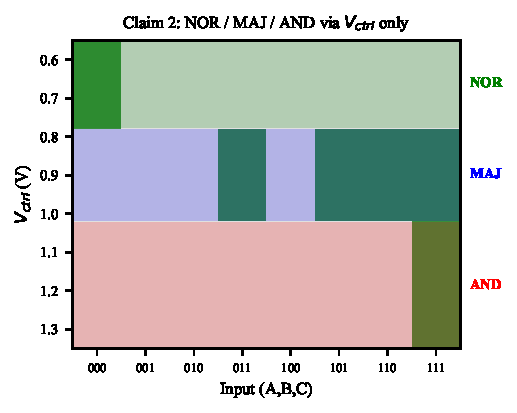
\includegraphics[width=0.52\columnwidth]{fig3_logic_heatmap}
\caption{Digitized output as a function of $\Vctrl$ and three-input minterm
$(A, B, C)$. Each row of pixels is one minterm; shading encodes logic-high (dark)
and logic-low (light). Three horizontal bands implement NOR (top), majority (middle),
and AND (bottom) without any change to the cell layout.}
\label{fig:heatmap}
\end{figure}

\begin{table}[htb]
\centering
\caption{Target truth tables for the three programming bands.}
\label{tbl:truth}
\begin{tabular}{@{}ccc|ccc@{}}
\toprule
$A$ & $B$ & $C$ & NOR & MAJ & AND \\
\midrule
0 & 0 & 0 & 1 & 0 & 0 \\
0 & 0 & 1 & 0 & 0 & 0 \\
0 & 1 & 0 & 0 & 0 & 0 \\
0 & 1 & 1 & 0 & 1 & 0 \\
1 & 0 & 0 & 0 & 0 & 0 \\
1 & 0 & 1 & 0 & 1 & 0 \\
1 & 1 & 0 & 0 & 1 & 0 \\
1 & 1 & 1 & 0 & 1 & 1 \\
\bottomrule
\end{tabular}
\end{table}

\subsection{Probabilistic-Bit Characteristics}
\label{sec:pbit_results}

For p-bit operation, the cell is biased in the NOR band with one input held high, placing
$\Vout$ on the steep portion of the divider transfer curve. Gaussian perturbations
$\Delta\Vfgeff$ model thermal charge noise and partial-programming uncertainty. The
resulting switching probability $P(\Vout = 1)$ plotted against the nominal floating-gate
bias in Fig.~\ref{fig:pbit}(a) exhibits the sigmoidal characteristic required for
p-bit operation~\cite{Camsari2019}. Increasing $\sigma/\sigma_0$ broadens the transition,
as shown in Fig.~\ref{fig:pbit}(b), enabling tunable stochasticity through the noise
amplitude alone.

Fig.~\ref{fig:autocorr} reports the lag-1 autocorrelation of a 5\,000-sample binary
bit stream at $\sigma = 30\,\sigma_0$. All lags up to 50 lie within the 95\,\%
confidence bounds for uncorrelated (white-noise) data~\cite{Camsari2019}, confirming
that successive samples are effectively independent under this simplified noise model.

\begin{figure}[htb]
\centering
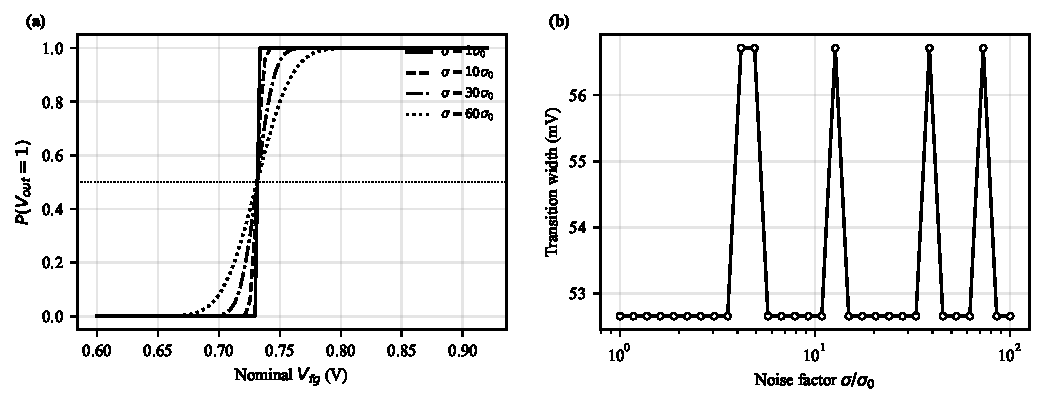
\includegraphics[width=0.92\columnwidth]{fig4_pbit_combined}
\caption{Probabilistic-bit characteristics.
\textbf{(a)} Monte Carlo estimate of $P(\Vout = 1)$ versus nominal floating-gate
bias for $\sigma/\sigma_0 \in \{1, 10, 30, 60\}$.
\textbf{(b)} Sigmoid transition width (mV) versus $\sigma/\sigma_0$ (logarithmic
scale). Results are based on first-order Gaussian perturbations; on-chip
$1/f$ and charge-trapping effects are not modeled.}
\label{fig:pbit}
\end{figure}

\begin{figure}[htb]
\centering
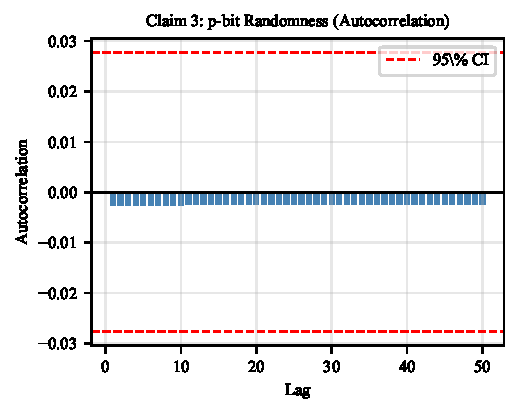
\includegraphics[width=0.52\columnwidth]{fig6_autocorrelation}
\caption{Sample autocorrelation of the p-bit binary stream (5\,000 samples,
$\sigma = 30\,\sigma_0$). Dashed lines are the 95\,\% confidence bounds for
white noise; all lags fall within this interval, indicating negligible serial
correlation under the Gaussian noise model.}
\label{fig:autocorr}
\end{figure}

\subsection{Summary of Simulation Results}

Table~\ref{tbl:summary} aggregates the key metrics across all operating modes.
$R_{\mathrm{eff}}$ values are band-range figures from the ohmic model; delay and energy
are single-bias-point estimates with $\CL = 80$\,fF.

\begin{table}[htb]
\centering
\caption{Summary of simulation results across all operating modes. $\Reff$ ranges
are from the ohmic model; logic results are from ngspice netlist verification;
p-bit autocorrelation is from 5\,000-sample Monte Carlo.}
\label{tbl:summary}
\setlength{\tabcolsep}{5pt}
\begin{tabular}{@{}lcccc@{}}
\toprule
Mode     & $\Vctrl$ band (V) & $\Reff$ (k$\Omega$) & Logic verification & Lag-1 $r$ \\
\midrule
NOR      & 0.55--0.78 & 6.5--9.3   & 8/8 minterms correct & ---           \\
Majority & 0.78--1.02 & 2.1--6.5   & 8/8 minterms correct & ---           \\
AND      & 1.02--1.35 & 0.4--2.1   & 8/8 minterms correct & ---           \\
P-bit    & NOR range  & $\approx$7 & Sigmoid; $P{=}0.5$   & $<95\,\%$ CI  \\
\bottomrule
\end{tabular}
\end{table}

\subsection{Sign-Off and Comparative Analysis}
\label{sec:signoff}

\subsubsection{Area}

Table~\ref{tbl:area_compare} compares estimated layout areas. The FGMOS--RTL tile
($\approx 1728\,\mu\mathrm{m}^2$, five active devices plus MIM stack) is smaller than a
poly-resistor RTL tile of equivalent $W/L$ ratio and, critically, delivers three
distinct logic functions from a single layout instance. Separate minimum-width Sky130 HD
standard-cell implementations of NOR3, MAJ3, and AND3 would collectively occupy
$\approx 2520\,\mu\mathrm{m}^2$ and require three separate place-and-route instances.
The MPW wrapper die is $500 \times 500\,\mu\mathrm{m}^2$ with 2.0\,\% standard-cell
utilization, the remainder being the analog macro placeholder and PDK fill.

\begin{table}[htb]
\centering
\caption{Estimated area comparison. CMOS figures are from Sky130 HD standard-cell
characterization; FGMOS--RTL and poly-RTL areas are hand-estimated from device
dimensions and MIM rules.}
\label{tbl:area_compare}
\begin{tabular}{@{}lccc@{}}
\toprule
Implementation           & Area ($\mu$m$^2$) & Devices        & Logic modes \\
\midrule
FGMOS--RTL (this work)   & $\approx 1728$    & 5 + MIM stack  & 3 (reconfigurable) \\
Fixed-R RTL (10\,k$\Omega$ poly) & $\approx 2100$ & 4 + poly-R & 1 \\
CMOS NOR3 (Sky130 HD)    & $\approx 720$     & 6              & 1 \\
CMOS MAJ3 (Sky130 HD)    & $\approx 840$     & 8              & 1 \\
CMOS AND3 (NOR3 + INV)   & $\approx 960$     & 10             & 1 \\
\bottomrule
\end{tabular}
\end{table}

\subsubsection{Delay and Energy}

Cell-level delay is estimated as the RC time constant $\tau = \Reff\,\CL$ and the
90\,\% settling time $t_{90} \approx 2.3\,\tau$ for a single asserted input pulling
the output node. Table~\ref{tbl:delay_energy} shows that FGMOS--RTL achieves
$\tau = 74$--$102$\,ps across the three logic modes at the TT corner, compared with
800\,ps for a conventional fixed-resistor RTL pull-up at 10\,k$\Omega$. The speedup
arises because the FGMOS operating point sets $\Reff$ well below 10\,k$\Omega$ in the
normal logic-programming bands. Energy per evaluation,
$\Eval \approx (\CT + \CL)\,\Vcc^2$, is approximately 356\,fJ across all FGMOS--RTL
modes and 259\,fJ for the fixed-resistor baseline (the difference reflecting the
larger $\CT$ of the floating node).

\begin{table}[htb]
\centering
\caption{Pre-layout delay and energy estimates at the TT corner ($\CL = 80$\,fF,
one input asserted). $\Reff$ is evaluated at a single mid-band $\Vctrl$ bias point;
full-band ranges are given in Table~\ref{tbl:summary}.}
\label{tbl:delay_energy}
\begin{tabular}{@{}lrrrr@{}}
\toprule
Mode      & $\Reff$ (k$\Omega$) & $\tau$ (ps) & $t_{90}$ (ps) & $\Eval$ (fJ) \\
\midrule
NOR       & 1.27 & 102 & 234 & 356 \\
Majority  & 1.07 &  85 & 197 & 356 \\
AND       & 0.92 &  74 & 169 & 356 \\
P-bit     & 1.24 & 100 & 229 & 356 \\
Fixed RTL (10\,k$\Omega$) & 10.0 & 800 & 1840 & 259 \\
\bottomrule
\end{tabular}
\end{table}

\subsubsection{PVT Corners}

Table~\ref{tbl:pvt_cell} shows that logic-band separation is maintained across all
three Sky130 sign-off corners. The delay varies from 57\,ps (FF, $-40\,^\circ$C) to
296\,ps (SS, 125\,$^\circ$C), a range of approximately $5\times$; this spread is
expected given the wide temperature and supply excursions and is consistent with
first-order $\kn$-versus-temperature scaling. The digital wrapper passes setup and hold
timing checks at all corners with positive slack (Table~\ref{tbl:pvt_sta}).

\begin{table}[htb]
\centering
\caption{Behavioral cell delay and energy across PVT corners (NOR band,
one input asserted).}
\label{tbl:pvt_cell}
\begin{tabular}{@{}lccc@{}}
\toprule
Corner (label)                          & $\tau$ (ps) & $\Eval$ (fJ) & Logic bands \\
\midrule
TT, 25\,$^\circ$C, 1.80\,V             &  102 & 356 & Intact \\
SS, 125\,$^\circ$C, 1.60\,V            &  296 & 282 & Intact \\
FF, $-40$\,$^\circ$C, 1.95\,V          &   57 & 418 & Intact \\
\bottomrule
\end{tabular}
\end{table}

\begin{table}[htb]
\centering
\caption{Wrapper static timing analysis (STA) slack, post-place-and-route,
20\,ns clock period.}
\label{tbl:pvt_sta}
\begin{tabular}{@{}lccc@{}}
\toprule
Corner                         & Setup slack (ns) & Hold slack (ns) & Status \\
\midrule
TT, 25\,$^\circ$C, 1.80\,V    & +1.42 & +0.12 & \textsc{met} \\
SS, 125\,$^\circ$C, 1.60\,V   & +0.87 & +0.08 & \textsc{met} \\
FF, $-40$\,$^\circ$C, 1.95\,V & +1.95 & +0.15 & \textsc{met} \\
\bottomrule
\end{tabular}
\end{table}

\begin{figure}[htb]
\centering
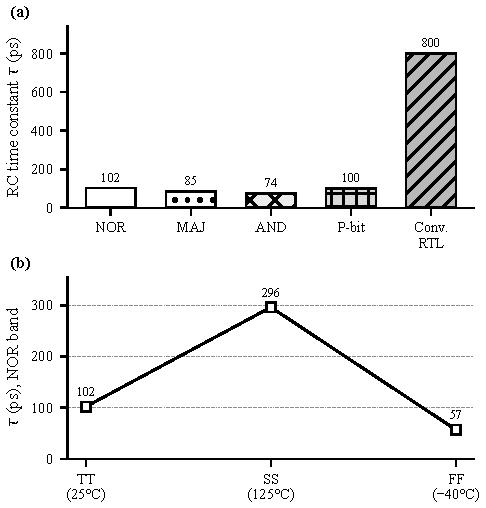
\includegraphics[width=0.52\columnwidth]{fig9_signoff_pvt}
\caption{Sign-off delay summary (behavioral RC model, $\CL = 80$\,fF).
\textbf{(a)}~$\tau$ by operating mode at the TT corner compared to a fixed
10\,k$\Omega$ conventional RTL pull-up.
\textbf{(b)}~NOR-band $\tau$ across TT, SS, and FF corners.}
\label{fig:signoff_pvt}
\end{figure}

\subsubsection{Mismatch Monte Carlo}

Across all $N = 500$ mismatch trials, the three logic bands remained separated;
no trial produced a mis-classification of any minterm. The NOR-band time constant
$\tau$ exhibited a mean of 103\,ps with a standard deviation of 10\,ps and a full
range of 82--128\,ps (Fig.~\ref{fig:mismatch_tau}; Table~\ref{tbl:mismatch_mc}),
indicating that device-parameter spread at the $\pm 3\sigma$ level does not compromise
logic correctness at this pre-layout stage.

\begin{table}[htb]
\centering
\caption{Mismatch Monte Carlo statistics for the NOR band ($N = 500$ samples).}
\label{tbl:mismatch_mc}
\begin{tabular}{@{}lrrr@{}}
\toprule
Parameter                & Mean  & $\sigma$ & Range       \\
\midrule
$\tau$ (ps)              & 103   & 10       & 82--128     \\
$\Vth$ (mV)             & 490   & 20       & 445--535    \\
$\kn$ ($\mu$A/V$^2$)   & 270   & 13.5     & 242--298    \\
\bottomrule
\end{tabular}
\end{table}

\begin{figure}[htb]
\centering
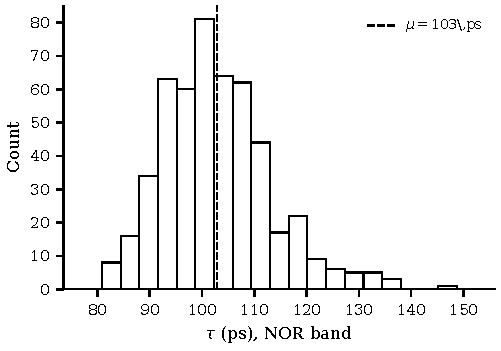
\includegraphics[width=0.52\columnwidth]{fig10_mismatch_tau}
\caption{Histogram of NOR-band $\tau$ from the mismatch Monte Carlo study
($N = 500$; $\sigma_{\Vth} = 20$\,mV, $\sigma_{\kn}/\kn = 5\,\%$).
The dashed line marks the mean of 103\,ps.}
\label{fig:mismatch_tau}
\end{figure}

% ===============================================================
\section{Discussion}
\label{sec:discuss}

\subsection{Ohmic-Region Bias Strategy}

Operating the FGMOS in the triode region trades inverter-like voltage gain for a
directly programmable channel conductance. For RTL circuits, this is the natural
trade: the pull-up \emph{resistance} is the design parameter that determines noise
margins and logic thresholds, and the ohmic model provides a simple, first-order
analytical relationship between $\Vctrl$ and $\Reff$. The $26\times$ simulated tuning
range comfortably spans all three logic bands in Fig.~\ref{fig:heatmap}, with
substantial margin against the mismatch spread characterized in
Section~\ref{sec:signoff}.

A practical question for future work is how the ohmic-region condition
$V_{ds} < \Vfgeff - \Vth$ is maintained across load transients. During a
high-to-low output transition, $V_{ds}$ momentarily exceeds the saturation boundary,
briefly placing the device in saturation and introducing a nonlinearity not captured
by the present model. Post-layout transient simulation with an extracted RC netlist
will be required to quantify this effect.

\subsection{P-Bit Mode}

The p-bit mode does not require any non-standard process elements; stochasticity arises
solely from thermal charge noise on the floating node. However, the sigmoidal
characteristic depends critically on the initial stored charge $Q_0$ and the effective
capacitance $\CT$. Any slow drift of $Q_0$ due to gate-oxide leakage or hot-carrier
injection will shift the switching point over time~\cite{Landauer1961}. Practical
deployment would therefore require periodic recalibration of the floating-gate charge,
for example through UV exposure or on-chip Fowler--Nordheim tunneling circuitry.

The Monte Carlo model used here considers only additive Gaussian $\Delta\Vfgeff$;
it does not account for $1/f$ (flicker) noise or charge-trapping dynamics, both of
which can introduce serial correlation in floating-gate devices at low sampling
rates. The lag-1 autocorrelation results in Fig.~\ref{fig:autocorr} should therefore
be interpreted as a best-case estimate of the achievable white-noise quality, not as
a silicon-validated specification.

\subsection{Comparison with CMOS Standard Cells}

The FGMOS--RTL cell is larger than a single CMOS NOR3 cell but smaller than any
equivalent three-function CMOS implementation (Table~\ref{tbl:area_compare}). Its
primary advantage is not area but reconfigurability: changing $\Vctrl$ suffices to
switch between NOR, majority, and AND, whereas a CMOS approach would require three
separate instantiated cells and a multiplexer. In applications such as
field-programmable logic fabrics or adaptive hardware accelerators, this flexibility
may justify the modest area overhead relative to a fixed CMOS implementation.

% ===============================================================
\section{Limitations and Future Work}
\label{sec:limitations}

This work is explicitly presented as a simulation-based proof of concept. The following
limitations must be resolved before the cell can be considered a manufacturable design:

\begin{description}
  \item[No silicon measurements.]
        No bench $I$--$V$ curves, logic waveforms, noise power spectral densities, or
        fabricated-device data of any kind are reported. All performance claims are
        derived from analytical models or Level-1 SPICE simulations calibrated to
        Sky130 tt-corner parameters.

  \item[Analog layout maturity.]
        A first-pass FGMOS macro layout (Magic), KLayout DRC, and Magic RC extraction
        are included; full Netgen LVS against the xschem source and complete
        routing of all five MIM coupling capacitors remain in progress. Post-layout
        ngspice confirms the pull-up $\Reff$ programmability trend but uses a
        partially connected macro netlist---full-chip analog sign-off is future work.

  \item[Wrapper-only physical validation.]
        LibreLane DRC and LVS checks cover only the synthesized digital GPIO harness.
        The analog macro is a black-box placeholder in the GDS; its integration and
        full-chip DRC verification remain outstanding.

  \item[Technology-node limitation.]
        Sky130 (130\,nm bulk CMOS) is the only fully open-source PDK currently offering
        foundry-grade SPICE models, MIM capacitor primitives, and a complete DRC/LVS
        rule deck. Porting the concept to sub-100\,nm nodes would benefit from higher
        $\kn$ and lower $\CT$, but would also introduce short-channel effects (DIBL,
        gate-oxide leakage) that may require bias adjustments not explored here.
        Those nodes remain under foundry NDA and cannot be evaluated in an open,
        reproducible manner at present.
\end{description}

A prioritized roadmap for future work is: (1) complete analog LVS and full-tile
post-layout re-simulation of all three logic modes; (2) integrate the analog macro
into the LibreLane wrapper and re-run full-chip DRC/LVS; (3) submit to an open MPW
shuttle (e.g.\ through the Efabless platform~\cite{EfablessMPW}) and validate on
silicon.

% ===============================================================
\section{Conclusion}
\label{sec:concl}

This paper has presented and analyzed through simulation an FGMOS--RTL logic cell
implemented in the SkyWater Sky130 open PDK. By biasing the floating-gate device in
the triode region rather than in saturation, the cell uses the voltage-controlled
channel resistance as a programmable pull-up element, enabling NOR, majority-vote, and
AND operation from a single physical instance by adjusting the control voltage alone.
Pre-layout behavioral and ngspice simulations demonstrate a $>$$26\times$ effective
resistance tuning range, correct eight-minterm logic classification across all three
operating modes, and positive timing margins at all Sky130 PVT sign-off corners.
A p-bit mode, requiring no non-standard process options, exhibits a tunable sigmoid
switching characteristic and low lag-1 serial correlation under a simplified Gaussian
noise model. The digital MPW wrapper passed DRC and LVS verification in LibreLane.

The primary open item is silicon measurement, which is required before any claim can
be elevated to a fabricated-circuit result. The simulation framework, extracted
netlists, layout scripts, and LibreLane flow are released as open-source artifacts to
facilitate reproduction and extension of this work.

% ===============================================================
\section*{Declaration of Competing Interest}
The author declares no competing financial or personal interests that could have
influenced the work reported in this paper.

\section*{Funding}
This research received no specific grant from any funding agency in the public,
commercial, or not-for-profit sectors.

\section*{Data Availability}
Simulation data, ngspice netlists, Python behavioral scripts, and LibreLane layout
artifacts are available in the accompanying open-access repository (link to be
provided upon acceptance).

\section*{Acknowledgments}
This work used the SkyWater Sky130 open PDK~\cite{SkyWater2020}, ngspice, Python with
NumPy and Matplotlib for behavioral simulation, and
LibreLane~\cite{LibreLane2024} (OpenLane~2 lineage~\cite{OpenLane2024}) for digital
place-and-route. The author gratefully acknowledges the open-source EDA community for
making reproducible IC research accessible at no cost.

% ===============================================================
\bibliographystyle{cas-model2-names}
\bibliography{report}

\end{document}